\documentclass[12pt,class=report,crop=false]{standalone}
\usepackage[screen]{../python}

\pagestyle{empty}

\begin{document}

% Commande spécifique
\newcommand{\badletter}[1]{\underline{\textcolor{red}{#1}}}



%====================================================================
\chapitre{L-système}
%====================================================================


Un \defi{L-système} est la donnée d'un mot initial et de règles de remplacement.
Voici un exemple avec le mot de départ et une seule règle : \\
\centerline{\mot{BgAdB} \qquad \mot{A} $\rightarrow$ \mot{ABA}}


Le \defi{$k$-ème itéré} du L-système s'obtient en appliquant $k$ fois la substitution au mot de départ.
Avec notre exemple :
\begin{itemize}
  \item Première itération. Le mot de départ est \mot{BgAdB}, la règle est \mot{A} $\rightarrow$ \mot{ABA} : on remplace le \mot{A} par \mot{ABA}. On obtient le mot \mot{BgABAdB}.
  
  \item Deuxième itération. On part du mot obtenu \mot{BgABAdB}, on remplace les deux \mot{A} par \mot{ABA} : on obtient le mot \mot{BgABABABAdB}.
  
  \item Le troisième itéré est \mot{BgABABABABABABABAdB}, etc.  
\end{itemize}


\newpage


Lorsqu'il y a deux règles (ou plus) il faut les appliquer en même temps.
Voici un exemple de L-système à deux règles :
 \\
\centerline{\mot{A} \qquad \mot{A} $\rightarrow$ \mot{BgA} \qquad \mot{B} $\rightarrow$ \mot{BB}}
Avec notre exemple :
\begin{itemize}
  \item Première itération. Le mot de départ est \mot{A}, on applique la première règle \mot{A} $\rightarrow$ \mot{BgA} (la seconde règle ne s'applique pas, car il n'y a pas encore de \mot{B}): on obtient le mot \mot{BgA}.
  
  \item Deuxième itération. On part du mot obtenu \mot{BgA}, on remplace les \mot{A} par \mot{BgA} et en même temps les \mot{B} par \mot{BB} : on obtient le mot \mot{BBgBgA}.
  
  \item Le troisième itéré est \mot{BBBBgBBgBgA}, etc.  
\end{itemize}



\newpage

On te donne un mot (par exemple \mot{AgAdAAdAdA}) dans lequel chaque lettre (lues de gauche à droite) correspond à une instruction pour la tortue \Python{}.

\begin{itemize}
  \item \mot{A} ou \mot{B} : avance d'une quantité fixée (en traçant),
  \item \mot{g} : tourne à gauche, sans avancer, d'un angle fixé (le plus souvent $90$ degrés),
  \item \mot{d} : tourne à droite d'un angle fixé.
\end{itemize}

Les autres caractères ne font rien. (On ajoutera d'autres commandes plus loin).


\begin{center}
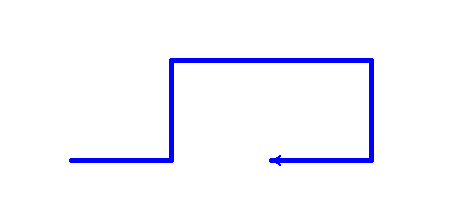
\includegraphics[scale=0.6]{ecran-lsysteme-1}
\end{center}
\end{document}
